\subsection{Beam Modeling} \label{sub:BeamModeling}
The beam model that will be utilized was developed by \citeauthor{Mandrekas1992} \cite{Mandrekas1992} for the "SuperCode". The model is based on a detailed quantum physics analysis to construct the cross-sections, but the implementation was simplified to a fit in \cref{eqn:beamxsection} based on the parameters:
\begin{itemize}
	\item Beam Energy, $E$ in keV/u,
	\item Beam particle atomic number, u
	\item Plasma Z-effective, $Z_{eff}$
	\item Electron Temperature, $T_e$ in keV, and
	\item Ion density, $n_e$ in $\text{cm}^{-3}$.
\end{itemize}
The primary cross-section function, $S_1$, is determined using \cref{eqn:beamS1} and the coefficients \cref{tab:BeamACoefficients}. Similarly, the impurity cross-section function, $S_z$ is calculated \cref{eqn:beamSz} with coefficients being shown in \cref{tab:BeamBCoefficients}. The sensitivity of the cross-section temperature for $Z_{eff}=1$ and $Z_{eff}=2$ are shown in \prettyref{fig:BeamXSecPrimaryTempSweep} and \prettyref{fig:BeamXSecImpurityTempSweep}, respectively. The sensitivity due to density is for the same $Z_{eff}$ are presented in \prettyref{fig:BeamXSecPrimaryDenSweep} and \prettyref{fig:BeamXSecImpurityDenSweep}.

The dominant physics for the beam energies, plasma densities and temperatures for tokamak plasmas are collisional radiative \cite{Janev1989}. 


\begin{equation}
	\sigma_s^{\left(z\right)}\left(E, n_e, T_e, Z_{eff}\right) = \cfrac{\exp\left[S_1\left(E, n_e, T_e\right)\right]}{E}
	\times \left[1 + \left(Z_{eff}-1\right) S_z\left(E, n_e, T_e\right) \right] \left(\times 10^{-16} \text{cm}^2 \right)
	\label{eqn:beamxsection}
\end{equation}
%
where
%
\begin{equation}
	S_1 = \sum_{i=1}^{2} \sum_{j=1}^{3} \sum_{k=1}^{2} \left\{ A_{ijk} \times \left(\ln E\right)^{i-1} 
	\left[ \ln \left(\cfrac{n}{n_0}\right) \right]^{j-1} \left( \ln T_e\right)^{k-1} \right\}
	\label{eqn:beamS1}
\end{equation}
%
and
%
\begin{equation}
	S_z = \sum_{i=1}^{3} \sum_{j=1}^{2} \sum_{k=1}^{2} \left\{ B_{ijk}^{\left(z\right)} \times \left(\ln E\right)^{i-1} 
	\left[ \ln \left(\cfrac{n}{n_0}\right) \right]^{j-1} \left( \ln T_e\right)^{k-1} \right\}
	\label{eqn:beamSz}
\end{equation}

\begin{table}
	\centering
	\caption{Values of fit coefficients\cite{Janev1989}}
	\subfloat[$A_{ijk}$ coefficients \newline \cref{eqn:beamS1}] {
		\begin{tabular}{|l|l|}
			\hline
			$ A_{ijk} $ &                                     \\
			\hline
			$ A_{111} $ & $\hphantom{-}4.40                $  \\
			$ A_{112} $ & $           -2.49 \times 10^{-2} $  \\ 
			$ A_{121} $ & $\hphantom{-}7.46 \times 10^{-2} $  \\ 
			$ A_{122} $ & $\hphantom{-}2.27 \times 10^{-3} $  \\ 
			$ A_{131} $ & $\hphantom{-}3.16 \times 10^{-3} $  \\ 
			$ A_{132} $ & $           -2.78 \times 10^{-5} $  \\
			$ A_{211} $ & $\hphantom{-}2.30 \times 10^{-1} $  \\
			$ A_{212} $ & $           -1.15 \times 10^{-2} $  \\
			$ A_{221} $ & $           -2.55 \times 10^{-3} $  \\
			$ A_{222} $ & $           -6.20 \times 10^{-4} $  \\
			$ A_{231} $ & $           -1.32 \times 10^{-3} $  \\
			\hline
		\end{tabular}	
		\label{tab:BeamACoefficients}
	} \quad
	\subfloat[$B_{ijk}$ coefficients for He, C, O and Fe Impurities \newline \cref{eqn:beamSz}] {
		\begin{tabular}{|l|c|c|c|c|}
			\hline
			$ B_{ijk}^{\left(z\right)}$ & He & C &  O & Fe \\
			\hline
			$ B_{111} $ & $           -2.36 \times 10^{0\hphantom{-}} $  
			            & $           -1.49 \times 10^{0\hphantom{-}} $ 
			            & $           -1.41 \times 10^{0\hphantom{-}} $ 
			            & $           -1.03 \times 10^{0\hphantom{-}} $ \\
			$ B_{112} $ & $\hphantom{-}1.85 \times 10^{-1} $  & $           -1.54 \times 10^{-2} $ &  $           -4.08 \times 10^{-4} $ & $\hphantom{-}1.06 \times 10^{-1} $ \\
			$ B_{121} $ & $           -2.50 \times 10^{-1} $  & $           -1.19 \times 10^{-1} $ &  $           -1.08 \times 10^{-1} $ & $           -5.58 \times 10^{-2} $ \\
			$ B_{122} $ & $           -3.81 \times 10^{-2} $  & $           -1.50 \times 10^{-2} $ &  $           -1.38 \times 10^{-2} $ & $           -3.72 \times 10^{-3} $ \\
			$ B_{211} $ & $\hphantom{-}8.49 \times 10^{-1} $  & $\hphantom{-}5.18 \times 10^{-1} $ &  $\hphantom{-}4.77 \times 10^{-1} $ & $\hphantom{-}3.22 \times 10^{-1} $ \\
			$ B_{212} $ & $           -4.78 \times 10^{-2} $  & $\hphantom{-}7.18 \times 10^{-3} $ &  $\hphantom{-}1.57 \times 10^{-3} $ & $           -3.75 \times 10^{-2} $ \\
			$ B_{221} $ & $\hphantom{-}6.77 \times 10^{-2} $  & $\hphantom{-}2.92 \times 10^{-2} $ &  $\hphantom{-}2.59 \times 10^{-2} $ & $\hphantom{-}1.24 \times 10^{-2} $ \\
			$ B_{222} $ & $\hphantom{-}1.05 \times 10^{-2} $  & $\hphantom{-}3.66 \times 10^{-3} $ &  $\hphantom{-}3.33 \times 10^{-3} $ & $\hphantom{-}8.61 \times 10^{-4} $ \\
			$ B_{311} $ & $           -5.88 \times 10^{-2} $  & $           -3.36 \times 10^{-2} $ &  $           -3.05 \times 10^{-2} $ & $           -1.87 \times 10^{-2} $ \\
			$ B_{312} $ & $\hphantom{-}4.34 \times 10^{-3} $  & $\hphantom{-}3.41 \times 10^{-4} $ &  $\hphantom{-}7.35 \times 10^{-4} $ & $\hphantom{-}3.53 \times 10^{-3} $ \\
			$ B_{321} $ & $           -4.48 \times 10^{-3} $  & $           -1.79 \times 10^{-3} $ &  $           -1.57 \times 10^{-3} $ & $           -7.43 \times 10^{-4} $ \\
			$ B_{322} $ & $           -6.76 \times 10^{-4} $  & $           -2.04 \times 10^{-4} $ &  $           -1.86 \times 10^{-4} $ & $           -5.12 \times 10^{-5} $ \\
			\hline
		\end{tabular}	
		\label{tab:BeamBCoefficients}
	}
\end{table}

\begin{figure}[!ht]
	\subfloat[$ Z_{eff} = 1 $] {
		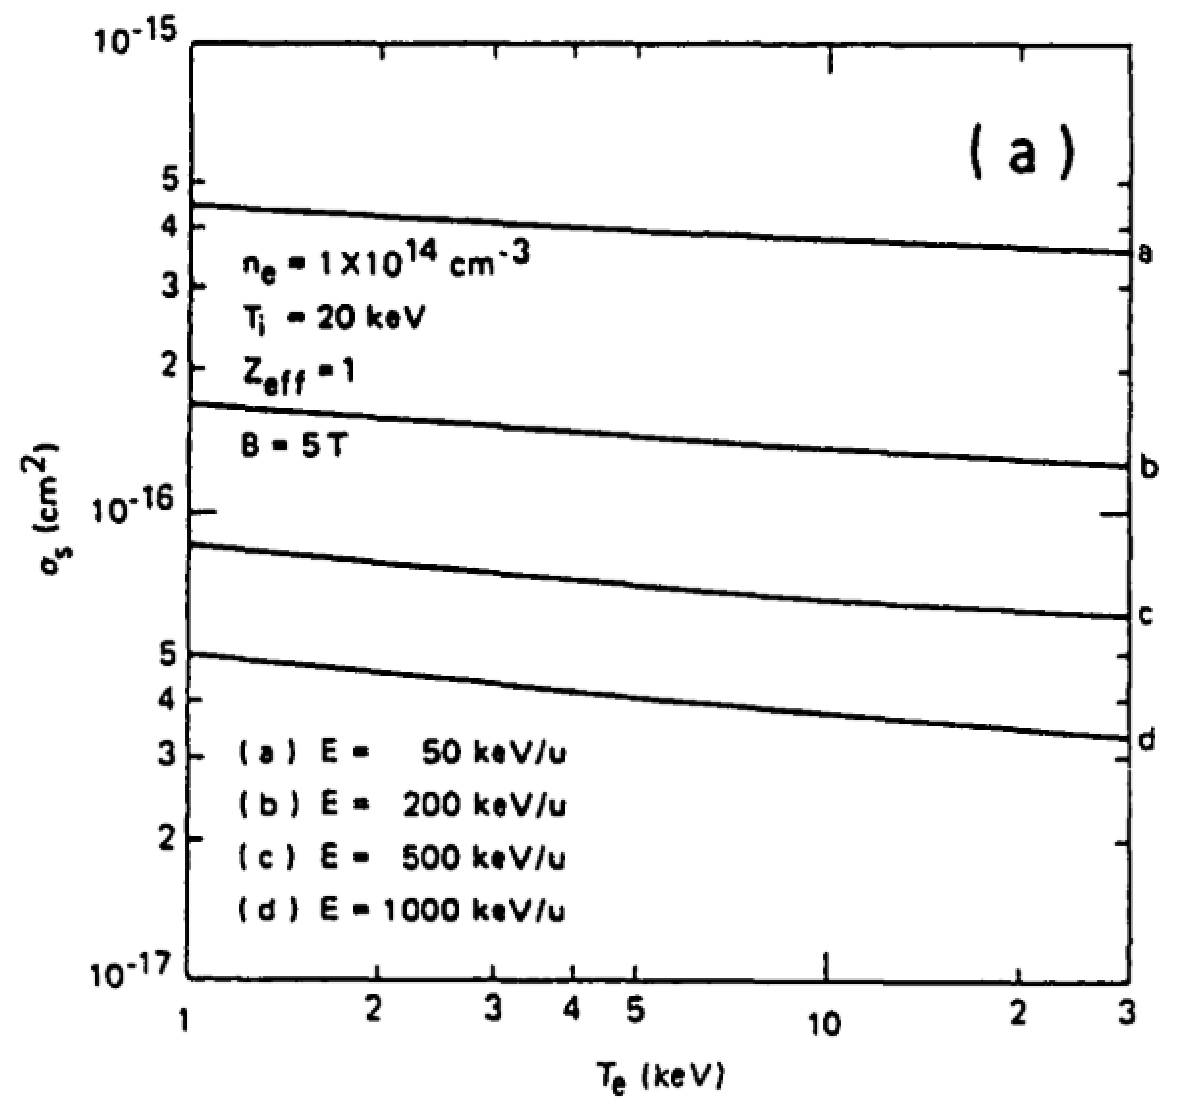
\includegraphics[width=0.45\linewidth]{images/beam_xsec_primary_temp_sweep}
		\label{fig:BeamXSecPrimaryTempSweep}
	} \quad
	\subfloat[$ Z_{eff} =2 $] {
		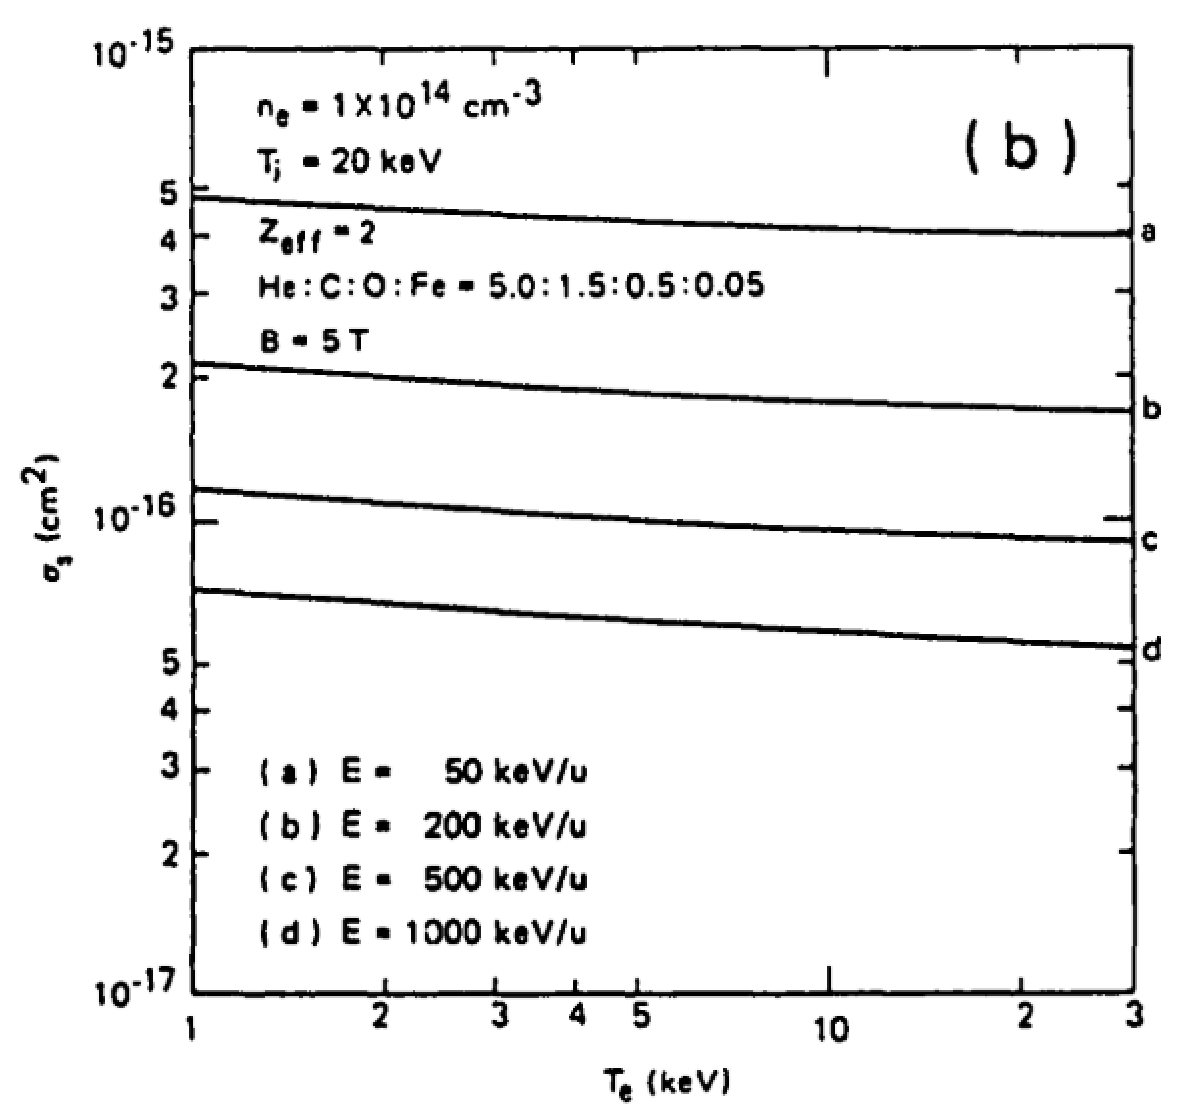
\includegraphics[width=0.45\linewidth]{images/beam_xsec_impurity_temp_sweep}
		\label{fig:BeamXSecImpurityTempSweep}
	}
	\caption{Temperature dependence of $\sigma_s$ for $n_e = 10^{14} \text{ cm}^{-3}$ for several beam energies \cite{Janev1989}}
\end{figure}


\begin{figure}[!ht]
	\subfloat[$ Z_{eff} = 1 $] {
		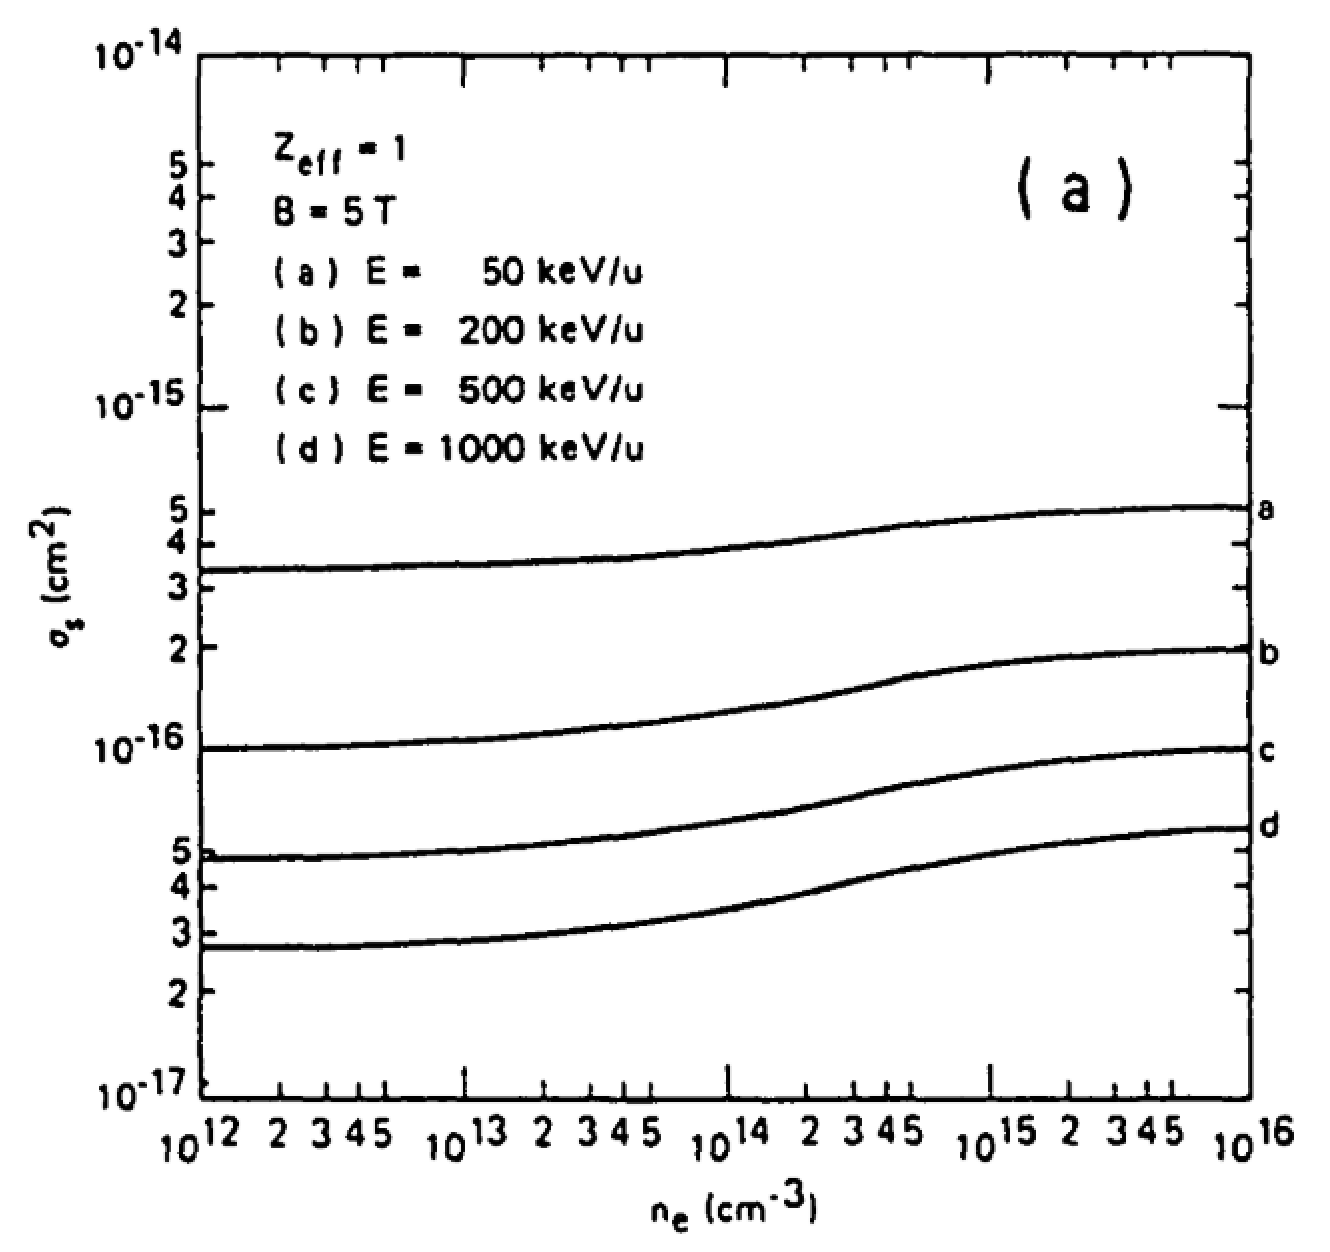
\includegraphics[width=0.45\linewidth]{images/beam_xsec_primary_den_sweep}
		\label{fig:BeamXSecPrimaryDenSweep}
	} \quad
	\subfloat[$ Z_{eff} =2 $] {
		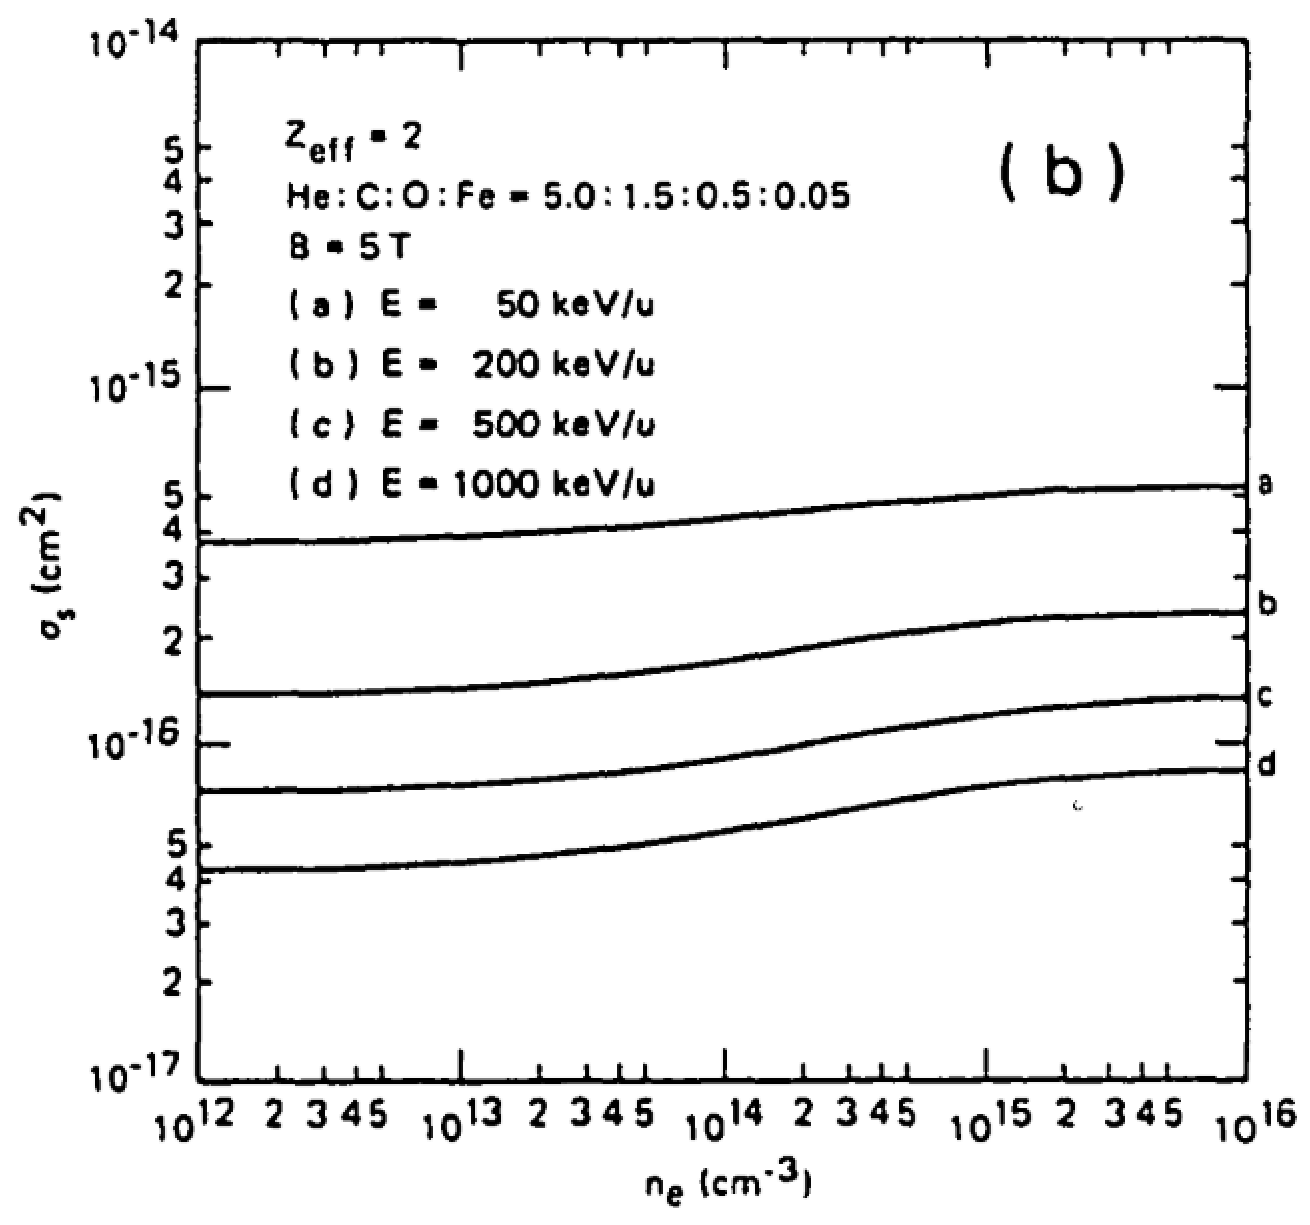
\includegraphics[width=0.45\linewidth]{images/beam_xsec_impurity_den_sweep}
		\label{fig:BeamXSecImpurityDenSweep}
	}
	\caption{Density dependence of $\sigma_s$ for several beam energies \cite{Janev1989}}
\end{figure}